% Options for packages loaded elsewhere
\PassOptionsToPackage{unicode}{hyperref}
\PassOptionsToPackage{hyphens}{url}
%
\documentclass[
]{article}
\usepackage{amsmath,amssymb}
\usepackage{lmodern}
\usepackage{iftex}
\ifPDFTeX
  \usepackage[T1]{fontenc}
  \usepackage[utf8]{inputenc}
  \usepackage{textcomp} % provide euro and other symbols
\else % if luatex or xetex
  \usepackage{unicode-math}
  \defaultfontfeatures{Scale=MatchLowercase}
  \defaultfontfeatures[\rmfamily]{Ligatures=TeX,Scale=1}
\fi
% Use upquote if available, for straight quotes in verbatim environments
\IfFileExists{upquote.sty}{\usepackage{upquote}}{}
\IfFileExists{microtype.sty}{% use microtype if available
  \usepackage[]{microtype}
  \UseMicrotypeSet[protrusion]{basicmath} % disable protrusion for tt fonts
}{}
\makeatletter
\@ifundefined{KOMAClassName}{% if non-KOMA class
  \IfFileExists{parskip.sty}{%
    \usepackage{parskip}
  }{% else
    \setlength{\parindent}{0pt}
    \setlength{\parskip}{6pt plus 2pt minus 1pt}}
}{% if KOMA class
  \KOMAoptions{parskip=half}}
\makeatother
\usepackage{xcolor}
\usepackage[margin=1in]{geometry}
\usepackage{color}
\usepackage{fancyvrb}
\newcommand{\VerbBar}{|}
\newcommand{\VERB}{\Verb[commandchars=\\\{\}]}
\DefineVerbatimEnvironment{Highlighting}{Verbatim}{commandchars=\\\{\}}
% Add ',fontsize=\small' for more characters per line
\usepackage{framed}
\definecolor{shadecolor}{RGB}{248,248,248}
\newenvironment{Shaded}{\begin{snugshade}}{\end{snugshade}}
\newcommand{\AlertTok}[1]{\textcolor[rgb]{0.94,0.16,0.16}{#1}}
\newcommand{\AnnotationTok}[1]{\textcolor[rgb]{0.56,0.35,0.01}{\textbf{\textit{#1}}}}
\newcommand{\AttributeTok}[1]{\textcolor[rgb]{0.77,0.63,0.00}{#1}}
\newcommand{\BaseNTok}[1]{\textcolor[rgb]{0.00,0.00,0.81}{#1}}
\newcommand{\BuiltInTok}[1]{#1}
\newcommand{\CharTok}[1]{\textcolor[rgb]{0.31,0.60,0.02}{#1}}
\newcommand{\CommentTok}[1]{\textcolor[rgb]{0.56,0.35,0.01}{\textit{#1}}}
\newcommand{\CommentVarTok}[1]{\textcolor[rgb]{0.56,0.35,0.01}{\textbf{\textit{#1}}}}
\newcommand{\ConstantTok}[1]{\textcolor[rgb]{0.00,0.00,0.00}{#1}}
\newcommand{\ControlFlowTok}[1]{\textcolor[rgb]{0.13,0.29,0.53}{\textbf{#1}}}
\newcommand{\DataTypeTok}[1]{\textcolor[rgb]{0.13,0.29,0.53}{#1}}
\newcommand{\DecValTok}[1]{\textcolor[rgb]{0.00,0.00,0.81}{#1}}
\newcommand{\DocumentationTok}[1]{\textcolor[rgb]{0.56,0.35,0.01}{\textbf{\textit{#1}}}}
\newcommand{\ErrorTok}[1]{\textcolor[rgb]{0.64,0.00,0.00}{\textbf{#1}}}
\newcommand{\ExtensionTok}[1]{#1}
\newcommand{\FloatTok}[1]{\textcolor[rgb]{0.00,0.00,0.81}{#1}}
\newcommand{\FunctionTok}[1]{\textcolor[rgb]{0.00,0.00,0.00}{#1}}
\newcommand{\ImportTok}[1]{#1}
\newcommand{\InformationTok}[1]{\textcolor[rgb]{0.56,0.35,0.01}{\textbf{\textit{#1}}}}
\newcommand{\KeywordTok}[1]{\textcolor[rgb]{0.13,0.29,0.53}{\textbf{#1}}}
\newcommand{\NormalTok}[1]{#1}
\newcommand{\OperatorTok}[1]{\textcolor[rgb]{0.81,0.36,0.00}{\textbf{#1}}}
\newcommand{\OtherTok}[1]{\textcolor[rgb]{0.56,0.35,0.01}{#1}}
\newcommand{\PreprocessorTok}[1]{\textcolor[rgb]{0.56,0.35,0.01}{\textit{#1}}}
\newcommand{\RegionMarkerTok}[1]{#1}
\newcommand{\SpecialCharTok}[1]{\textcolor[rgb]{0.00,0.00,0.00}{#1}}
\newcommand{\SpecialStringTok}[1]{\textcolor[rgb]{0.31,0.60,0.02}{#1}}
\newcommand{\StringTok}[1]{\textcolor[rgb]{0.31,0.60,0.02}{#1}}
\newcommand{\VariableTok}[1]{\textcolor[rgb]{0.00,0.00,0.00}{#1}}
\newcommand{\VerbatimStringTok}[1]{\textcolor[rgb]{0.31,0.60,0.02}{#1}}
\newcommand{\WarningTok}[1]{\textcolor[rgb]{0.56,0.35,0.01}{\textbf{\textit{#1}}}}
\usepackage{graphicx}
\makeatletter
\def\maxwidth{\ifdim\Gin@nat@width>\linewidth\linewidth\else\Gin@nat@width\fi}
\def\maxheight{\ifdim\Gin@nat@height>\textheight\textheight\else\Gin@nat@height\fi}
\makeatother
% Scale images if necessary, so that they will not overflow the page
% margins by default, and it is still possible to overwrite the defaults
% using explicit options in \includegraphics[width, height, ...]{}
\setkeys{Gin}{width=\maxwidth,height=\maxheight,keepaspectratio}
% Set default figure placement to htbp
\makeatletter
\def\fps@figure{htbp}
\makeatother
\setlength{\emergencystretch}{3em} % prevent overfull lines
\providecommand{\tightlist}{%
  \setlength{\itemsep}{0pt}\setlength{\parskip}{0pt}}
\setcounter{secnumdepth}{-\maxdimen} % remove section numbering
\ifLuaTeX
  \usepackage{selnolig}  % disable illegal ligatures
\fi
\IfFileExists{bookmark.sty}{\usepackage{bookmark}}{\usepackage{hyperref}}
\IfFileExists{xurl.sty}{\usepackage{xurl}}{} % add URL line breaks if available
\urlstyle{same} % disable monospaced font for URLs
\hypersetup{
  pdftitle={Peer Assesment 1: PA1\_template},
  pdfauthor={Julia E. Neidhardt},
  hidelinks,
  pdfcreator={LaTeX via pandoc}}

\title{Peer Assesment 1: PA1\_template}
\author{Julia E. Neidhardt}
\date{2023-06-29}

\begin{document}
\maketitle

\hypertarget{loading-libraries}{%
\section{Loading Libraries}\label{loading-libraries}}

\begin{Shaded}
\begin{Highlighting}[]
\CommentTok{\# Loading and processing the data begins with loading packages and libraries}
\FunctionTok{library}\NormalTok{(dplyr)}
\end{Highlighting}
\end{Shaded}

\begin{verbatim}
## Warning: package 'dplyr' was built under R version 4.3.1
\end{verbatim}

\begin{verbatim}
## 
## Attaching package: 'dplyr'
\end{verbatim}

\begin{verbatim}
## The following objects are masked from 'package:stats':
## 
##     filter, lag
\end{verbatim}

\begin{verbatim}
## The following objects are masked from 'package:base':
## 
##     intersect, setdiff, setequal, union
\end{verbatim}

\begin{Shaded}
\begin{Highlighting}[]
\FunctionTok{library}\NormalTok{(tidyverse)}
\end{Highlighting}
\end{Shaded}

\begin{verbatim}
## Warning: package 'tidyverse' was built under R version 4.3.1
\end{verbatim}

\begin{verbatim}
## Warning: package 'ggplot2' was built under R version 4.3.1
\end{verbatim}

\begin{verbatim}
## Warning: package 'lubridate' was built under R version 4.3.1
\end{verbatim}

\begin{verbatim}
## -- Attaching core tidyverse packages ------------------------ tidyverse 2.0.0 --
## v forcats   1.0.0     v readr     2.1.4
## v ggplot2   3.4.2     v stringr   1.5.0
## v lubridate 1.9.2     v tibble    3.2.1
## v purrr     1.0.1     v tidyr     1.3.0
\end{verbatim}

\begin{verbatim}
## -- Conflicts ------------------------------------------ tidyverse_conflicts() --
## x dplyr::filter() masks stats::filter()
## x dplyr::lag()    masks stats::lag()
## i Use the conflicted package (<http://conflicted.r-lib.org/>) to force all conflicts to become errors
\end{verbatim}

\begin{Shaded}
\begin{Highlighting}[]
\FunctionTok{library}\NormalTok{(ggplot2)}
\FunctionTok{library}\NormalTok{(knitr)}
\FunctionTok{library}\NormalTok{(rmarkdown)}
\end{Highlighting}
\end{Shaded}

\begin{verbatim}
## Warning: package 'rmarkdown' was built under R version 4.3.1
\end{verbatim}

\hypertarget{set-wd}{%
\section{Set WD}\label{set-wd}}

\begin{Shaded}
\begin{Highlighting}[]
\FunctionTok{setwd}\NormalTok{(}\StringTok{"C:/Users/Owner/Documents/DataScience/ReproducibleResearch/PeerAssesment"}\NormalTok{)}
\end{Highlighting}
\end{Shaded}

\hypertarget{load-and-test-data}{%
\section{Load and test data}\label{load-and-test-data}}

\begin{Shaded}
\begin{Highlighting}[]
\NormalTok{data }\OtherTok{\textless{}{-}} \FunctionTok{read.csv}\NormalTok{(}\StringTok{"C:/Users/Owner/Documents/DataScience/ReproducibleResearch/PeerAssesment/activity.csv"}\NormalTok{)}
\CommentTok{\# Display the first few rows of the data frame to ensure the data has processed correctly.}
\FunctionTok{head}\NormalTok{(data)}
\end{Highlighting}
\end{Shaded}

\begin{verbatim}
##   steps      date interval
## 1    NA 10/1/2012        0
## 2    NA 10/1/2012        5
## 3    NA 10/1/2012       10
## 4    NA 10/1/2012       15
## 5    NA 10/1/2012       20
## 6    NA 10/1/2012       25
\end{verbatim}

\begin{Shaded}
\begin{Highlighting}[]
\FunctionTok{summary}\NormalTok{(data)}
\end{Highlighting}
\end{Shaded}

\begin{verbatim}
##      steps            date              interval     
##  Min.   :  0.00   Length:17568       Min.   :   0.0  
##  1st Qu.:  0.00   Class :character   1st Qu.: 588.8  
##  Median :  0.00   Mode  :character   Median :1177.5  
##  Mean   : 37.38                      Mean   :1177.5  
##  3rd Qu.: 12.00                      3rd Qu.:1766.2  
##  Max.   :806.00                      Max.   :2355.0  
##  NA's   :2304
\end{verbatim}

\begin{Shaded}
\begin{Highlighting}[]
\FunctionTok{plot}\NormalTok{(data}\SpecialCharTok{$}\NormalTok{steps }\SpecialCharTok{\textasciitilde{}}\NormalTok{ data}\SpecialCharTok{$}\NormalTok{interval)}
\end{Highlighting}
\end{Shaded}

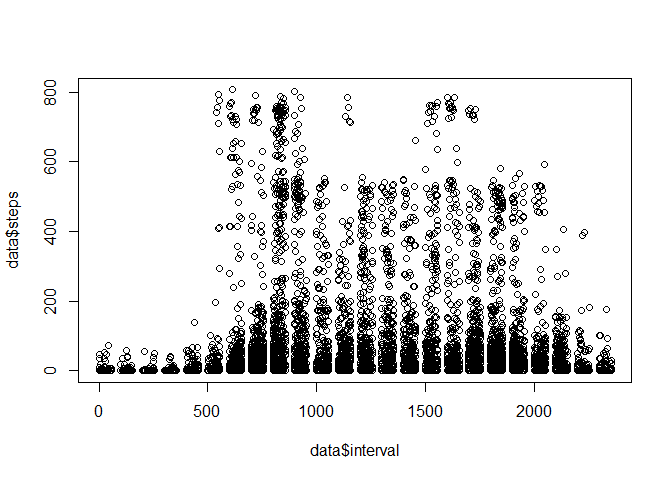
\includegraphics{PA1_template_files/figure-latex/number_of_steps_per_interval-1.pdf}
\# Calculate total steps per day

\begin{Shaded}
\begin{Highlighting}[]
\NormalTok{total\_steps\_per\_day }\OtherTok{\textless{}{-}} \FunctionTok{aggregate}\NormalTok{(data}\SpecialCharTok{$}\NormalTok{steps, }\AttributeTok{by=}\FunctionTok{list}\NormalTok{(}\AttributeTok{date=}\NormalTok{data}\SpecialCharTok{$}\NormalTok{date), }\AttributeTok{FUN=}\NormalTok{sum, }\AttributeTok{na.rm=}\ConstantTok{TRUE}\NormalTok{)}
\FunctionTok{names}\NormalTok{(total\_steps\_per\_day) }\OtherTok{\textless{}{-}} \FunctionTok{c}\NormalTok{(}\StringTok{"date"}\NormalTok{, }\StringTok{"total\_steps"}\NormalTok{)}
\end{Highlighting}
\end{Shaded}

\hypertarget{what-are-the-total-number-of-steps-taken-each-day}{%
\section{What are the total number of steps taken each
day?}\label{what-are-the-total-number-of-steps-taken-each-day}}

\begin{Shaded}
\begin{Highlighting}[]
\NormalTok{total\_steps\_per\_day }\OtherTok{\textless{}{-}}\NormalTok{ data }\SpecialCharTok{\%\textgreater{}\%} 
  \FunctionTok{group\_by}\NormalTok{(date) }\SpecialCharTok{\%\textgreater{}\%} 
  \FunctionTok{summarise}\NormalTok{(}\AttributeTok{total\_steps =} \FunctionTok{sum}\NormalTok{(steps, }\AttributeTok{na.rm =} \ConstantTok{TRUE}\NormalTok{))}
\end{Highlighting}
\end{Shaded}

\hypertarget{printing-the-first-few-rows-of-the-total_steps_per_day-dataframe-to-check-if-its-created-properly}{%
\section{\# Printing the first few rows of the total\_steps\_per\_day
dataframe to check if it's created
properly}\label{printing-the-first-few-rows-of-the-total_steps_per_day-dataframe-to-check-if-its-created-properly}}

\begin{Shaded}
\begin{Highlighting}[]
\FunctionTok{head}\NormalTok{(total\_steps\_per\_day)}
\end{Highlighting}
\end{Shaded}

\begin{verbatim}
## # A tibble: 6 x 2
##   date       total_steps
##   <chr>            <int>
## 1 10/1/2012            0
## 2 10/10/2012        9900
## 3 10/11/2012       10304
## 4 10/12/2012       17382
## 5 10/13/2012       12426
## 6 10/14/2012       15098
\end{verbatim}

\hypertarget{what-are-the-total-number-of-steps-taken-per-day}{%
\section{What are the Total Number of Steps Taken per
Day?}\label{what-are-the-total-number-of-steps-taken-per-day}}

\begin{Shaded}
\begin{Highlighting}[]
\CommentTok{\# Create the plot with a title}
\NormalTok{scatter\_plot }\OtherTok{\textless{}{-}} \FunctionTok{ggplot}\NormalTok{(total\_steps\_per\_day, }\FunctionTok{aes}\NormalTok{(}\AttributeTok{x=}\NormalTok{date, }\AttributeTok{y=}\NormalTok{total\_steps)) }\SpecialCharTok{+}
  \FunctionTok{geom\_point}\NormalTok{() }\SpecialCharTok{+}
  \FunctionTok{labs}\NormalTok{(}\AttributeTok{title =} \StringTok{"Total Steps per Day"}\NormalTok{, }\AttributeTok{x =} \StringTok{"Date"}\NormalTok{, }\AttributeTok{y =} \StringTok{"Total Steps"}\NormalTok{)}

\CommentTok{\# Print the plot}
\FunctionTok{print}\NormalTok{(scatter\_plot)}
\end{Highlighting}
\end{Shaded}

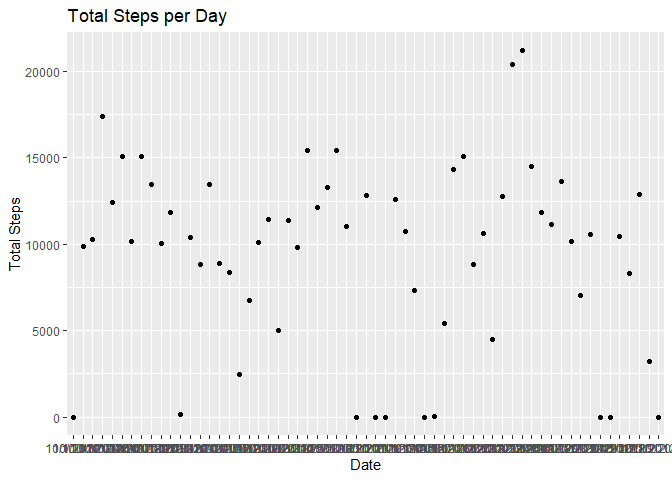
\includegraphics{PA1_template_files/figure-latex/steps_per_day_plot-1.pdf}

\begin{Shaded}
\begin{Highlighting}[]
\CommentTok{\# Save the plot to your working directory}
\FunctionTok{ggsave}\NormalTok{(}\StringTok{"total\_steps\_per\_day\_plot.png"}\NormalTok{, scatter\_plot)}
\end{Highlighting}
\end{Shaded}

\begin{verbatim}
## Saving 6.5 x 4.5 in image
\end{verbatim}

\hypertarget{mean-and-median-number-of-steps-taken-each-day}{%
\section{Mean and median number of steps taken each
day}\label{mean-and-median-number-of-steps-taken-each-day}}

\begin{Shaded}
\begin{Highlighting}[]
\CommentTok{\# Calculate mean and median steps per day}
\NormalTok{mean\_steps\_per\_day }\OtherTok{\textless{}{-}} \FunctionTok{mean}\NormalTok{(total\_steps\_per\_day}\SpecialCharTok{$}\NormalTok{total\_steps, }\AttributeTok{na.rm =} \ConstantTok{TRUE}\NormalTok{)}
\NormalTok{median\_steps\_per\_day }\OtherTok{\textless{}{-}} \FunctionTok{median}\NormalTok{(total\_steps\_per\_day}\SpecialCharTok{$}\NormalTok{total\_steps, }\AttributeTok{na.rm =} \ConstantTok{TRUE}\NormalTok{)}

\NormalTok{mean\_steps\_per\_day}
\end{Highlighting}
\end{Shaded}

\begin{verbatim}
## [1] 9354.23
\end{verbatim}

\begin{Shaded}
\begin{Highlighting}[]
\NormalTok{median\_steps\_per\_day}
\end{Highlighting}
\end{Shaded}

\begin{verbatim}
## [1] 10395
\end{verbatim}

\hypertarget{create-a-histogram-of-the-total-number-of-steps-taken-per-day}{%
\section{Create a histogram of the total number of steps taken per
day}\label{create-a-histogram-of-the-total-number-of-steps-taken-per-day}}

\begin{Shaded}
\begin{Highlighting}[]
\CommentTok{\# Create the histogram and add vertical lines for mean and median}
\NormalTok{hist\_plot }\OtherTok{\textless{}{-}} \FunctionTok{ggplot}\NormalTok{(total\_steps\_per\_day, }\FunctionTok{aes}\NormalTok{(}\AttributeTok{x=}\NormalTok{total\_steps)) }\SpecialCharTok{+}
  \FunctionTok{geom\_histogram}\NormalTok{(}\AttributeTok{binwidth =} \DecValTok{1000}\NormalTok{, }\AttributeTok{fill =} \StringTok{"blue"}\NormalTok{, }\AttributeTok{color =} \StringTok{"black"}\NormalTok{) }\SpecialCharTok{+}
  \FunctionTok{geom\_vline}\NormalTok{(}\FunctionTok{aes}\NormalTok{(}\AttributeTok{xintercept=}\NormalTok{mean\_steps\_per\_day), }\AttributeTok{color=}\StringTok{"red"}\NormalTok{, }\AttributeTok{linetype=}\StringTok{"dashed"}\NormalTok{, }\AttributeTok{size=}\DecValTok{1}\NormalTok{) }\SpecialCharTok{+}
  \FunctionTok{geom\_vline}\NormalTok{(}\FunctionTok{aes}\NormalTok{(}\AttributeTok{xintercept=}\NormalTok{median\_steps\_per\_day), }\AttributeTok{color=}\StringTok{"green"}\NormalTok{, }\AttributeTok{linetype=}\StringTok{"dashed"}\NormalTok{, }\AttributeTok{size=}\DecValTok{1}\NormalTok{) }\SpecialCharTok{+}
  \FunctionTok{labs}\NormalTok{(}\AttributeTok{title=}\StringTok{"Histogram of Total Steps per Day"}\NormalTok{, }\AttributeTok{x=}\StringTok{"Total Steps"}\NormalTok{, }\AttributeTok{y=}\StringTok{"Frequency"}\NormalTok{) }\SpecialCharTok{+}
  \FunctionTok{annotate}\NormalTok{(}\StringTok{"text"}\NormalTok{, }\AttributeTok{x =}\NormalTok{ mean\_steps\_per\_day, }\AttributeTok{y =} \DecValTok{10}\NormalTok{, }\AttributeTok{label =} \StringTok{"Mean"}\NormalTok{, }\AttributeTok{color =} \StringTok{"red"}\NormalTok{) }\SpecialCharTok{+}
  \FunctionTok{annotate}\NormalTok{(}\StringTok{"text"}\NormalTok{, }\AttributeTok{x =}\NormalTok{ median\_steps\_per\_day, }\AttributeTok{y =} \DecValTok{20}\NormalTok{, }\AttributeTok{label =} \StringTok{"Median"}\NormalTok{, }\AttributeTok{color =} \StringTok{"green"}\NormalTok{)}
\end{Highlighting}
\end{Shaded}

\begin{verbatim}
## Warning: Using `size` aesthetic for lines was deprecated in ggplot2 3.4.0.
## i Please use `linewidth` instead.
## This warning is displayed once every 8 hours.
## Call `lifecycle::last_lifecycle_warnings()` to see where this warning was
## generated.
\end{verbatim}

\begin{Shaded}
\begin{Highlighting}[]
\CommentTok{\# Print the plot}
\FunctionTok{print}\NormalTok{(hist\_plot)}
\end{Highlighting}
\end{Shaded}

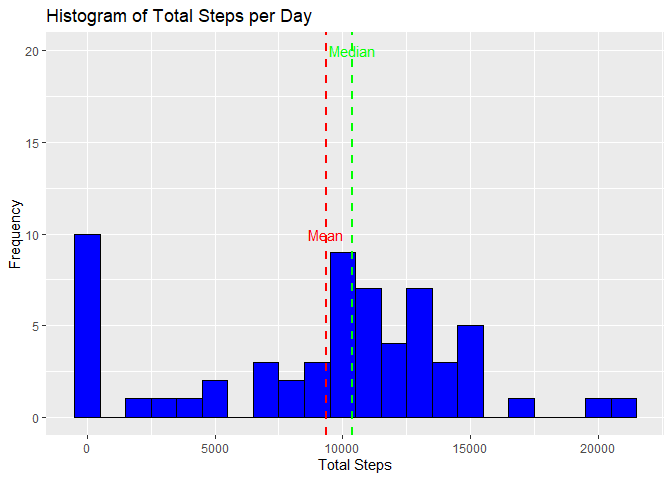
\includegraphics{PA1_template_files/figure-latex/histogram_of_total_steps_per_day-1.pdf}

\begin{Shaded}
\begin{Highlighting}[]
\CommentTok{\# Save the plot}
\FunctionTok{ggsave}\NormalTok{(}\StringTok{"histogram\_plot.png"}\NormalTok{, hist\_plot)}
\end{Highlighting}
\end{Shaded}

\begin{verbatim}
## Saving 6.5 x 4.5 in image
\end{verbatim}

\hypertarget{create-a-time-series-plot-for-total-steps-per-day}{%
\section{Create a time series plot for total steps per
day}\label{create-a-time-series-plot-for-total-steps-per-day}}

\begin{Shaded}
\begin{Highlighting}[]
\CommentTok{\# Check the structure of data first so as not to confuse poor R}
\FunctionTok{str}\NormalTok{(total\_steps\_per\_day)}
\end{Highlighting}
\end{Shaded}

\begin{verbatim}
## tibble [61 x 2] (S3: tbl_df/tbl/data.frame)
##  $ date       : chr [1:61] "10/1/2012" "10/10/2012" "10/11/2012" "10/12/2012" ...
##  $ total_steps: int [1:61] 0 9900 10304 17382 12426 15098 10139 15084 13452 10056 ...
\end{verbatim}

\begin{Shaded}
\begin{Highlighting}[]
\CommentTok{\# Then, convert \textquotesingle{}date\textquotesingle{} to Date class if it\textquotesingle{}s not already formatted as such}
\NormalTok{total\_steps\_per\_day}\SpecialCharTok{$}\NormalTok{date }\OtherTok{\textless{}{-}} \FunctionTok{as.Date}\NormalTok{(total\_steps\_per\_day}\SpecialCharTok{$}\NormalTok{date)}

\CommentTok{\# Next, calculate average of total steps per day}
\NormalTok{average\_steps }\OtherTok{\textless{}{-}} \FunctionTok{mean}\NormalTok{(total\_steps\_per\_day}\SpecialCharTok{$}\NormalTok{total\_steps, }\AttributeTok{na.rm =} \ConstantTok{TRUE}\NormalTok{)}

\NormalTok{time\_series\_plot }\OtherTok{\textless{}{-}} \FunctionTok{ggplot}\NormalTok{(total\_steps\_per\_day, }\FunctionTok{aes}\NormalTok{(}\AttributeTok{x =}\NormalTok{ date, }\AttributeTok{y =}\NormalTok{ total\_steps)) }\SpecialCharTok{+}
  \FunctionTok{geom\_line}\NormalTok{(}\AttributeTok{na.rm =} \ConstantTok{TRUE}\NormalTok{) }\SpecialCharTok{+}  \CommentTok{\# set na.rm = TRUE to remove NA values}
  \FunctionTok{geom\_hline}\NormalTok{(}\AttributeTok{yintercept =}\NormalTok{ average\_steps, }\AttributeTok{color =} \StringTok{"red"}\NormalTok{, }\AttributeTok{linetype =} \StringTok{"dashed"}\NormalTok{) }\SpecialCharTok{+}  \CommentTok{\# add horizontal line at the average steps}
  \FunctionTok{labs}\NormalTok{(}\AttributeTok{title =} \StringTok{"Time Series of Total Steps per Day with Hline at the Average Steps"}\NormalTok{, }\AttributeTok{x =} \StringTok{"Date"}\NormalTok{, }\AttributeTok{y =} \StringTok{"Total Steps"}\NormalTok{) }\SpecialCharTok{+}
  \FunctionTok{annotate}\NormalTok{(}\StringTok{"text"}\NormalTok{, }\AttributeTok{x =} \FunctionTok{min}\NormalTok{(total\_steps\_per\_day}\SpecialCharTok{$}\NormalTok{date), }\AttributeTok{y =}\NormalTok{ average\_steps, }\AttributeTok{label =} \FunctionTok{paste}\NormalTok{(}\StringTok{"Average ="}\NormalTok{, }\FunctionTok{round}\NormalTok{(average\_steps)), }\AttributeTok{hjust =} \SpecialCharTok{{-}}\FloatTok{0.1}\NormalTok{, }\AttributeTok{color =} \StringTok{"red"}\NormalTok{)  }\CommentTok{\# add text to the average line}

\CommentTok{\# Display the plot}
\FunctionTok{print}\NormalTok{(time\_series\_plot)}
\end{Highlighting}
\end{Shaded}

\begin{verbatim}
## Warning: Removed 1 rows containing missing values (`geom_text()`).
\end{verbatim}

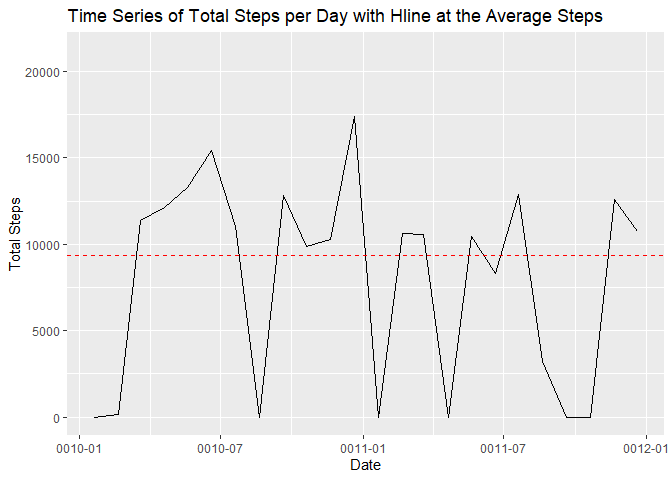
\includegraphics{PA1_template_files/figure-latex/time_series_plot_for_total_steps_per_day-1.pdf}

\begin{Shaded}
\begin{Highlighting}[]
\CommentTok{\# Save the plot}
\FunctionTok{ggsave}\NormalTok{(}\StringTok{"time\_series\_plot.png"}\NormalTok{, time\_series\_plot)}
\end{Highlighting}
\end{Shaded}

\begin{verbatim}
## Saving 6.5 x 4.5 in image
\end{verbatim}

\begin{verbatim}
## Warning: Removed 1 rows containing missing values (`geom_text()`).
\end{verbatim}

\hypertarget{time-series-plot-of-the-average-number-of-steps-taken}{%
\section{Time series plot of the average number of steps
taken}\label{time-series-plot-of-the-average-number-of-steps-taken}}

\begin{Shaded}
\begin{Highlighting}[]
\NormalTok{average\_steps\_per\_interval }\OtherTok{\textless{}{-}}\NormalTok{ data }\SpecialCharTok{\%\textgreater{}\%} 
  \FunctionTok{group\_by}\NormalTok{(interval) }\SpecialCharTok{\%\textgreater{}\%} 
  \FunctionTok{summarise}\NormalTok{(}\AttributeTok{avg\_steps =} \FunctionTok{mean}\NormalTok{(steps, }\AttributeTok{na.rm =} \ConstantTok{TRUE}\NormalTok{))}

\NormalTok{max\_steps\_interval }\OtherTok{\textless{}{-}}\NormalTok{ average\_steps\_per\_interval}\SpecialCharTok{$}\NormalTok{interval[}\FunctionTok{which.max}\NormalTok{(average\_steps\_per\_interval}\SpecialCharTok{$}\NormalTok{avg\_steps)]}

\FunctionTok{ggplot}\NormalTok{(average\_steps\_per\_interval, }\FunctionTok{aes}\NormalTok{(}\AttributeTok{x=}\NormalTok{interval, }\AttributeTok{y=}\NormalTok{avg\_steps)) }\SpecialCharTok{+}
  \FunctionTok{geom\_line}\NormalTok{(}\AttributeTok{color =} \StringTok{"blue"}\NormalTok{) }\SpecialCharTok{+}
  \FunctionTok{geom\_vline}\NormalTok{(}\FunctionTok{aes}\NormalTok{(}\AttributeTok{xintercept =}\NormalTok{ max\_steps\_interval), }\AttributeTok{color =} \StringTok{"red"}\NormalTok{, }\AttributeTok{linetype =} \StringTok{"dashed"}\NormalTok{, }\AttributeTok{size =} \DecValTok{1}\NormalTok{) }\SpecialCharTok{+}
  \FunctionTok{labs}\NormalTok{(}\AttributeTok{title=}\StringTok{"Time Series Plot of Average Steps per Interval: Max Avg Interval Noted"}\NormalTok{, }\AttributeTok{x=}\StringTok{"Interval"}\NormalTok{, }\AttributeTok{y=}\StringTok{"Average Steps"}\NormalTok{) }\SpecialCharTok{+}
  \FunctionTok{annotate}\NormalTok{(}\StringTok{"text"}\NormalTok{, }\AttributeTok{x =}\NormalTok{ max\_steps\_interval, }\AttributeTok{y =} \FunctionTok{max}\NormalTok{(average\_steps\_per\_interval}\SpecialCharTok{$}\NormalTok{avg\_steps), }\AttributeTok{label =} \StringTok{"Max Avg Interval"}\NormalTok{, }\AttributeTok{hjust =} \SpecialCharTok{{-}}\FloatTok{0.1}\NormalTok{, }\AttributeTok{color =} \StringTok{"red"}\NormalTok{)}
\end{Highlighting}
\end{Shaded}

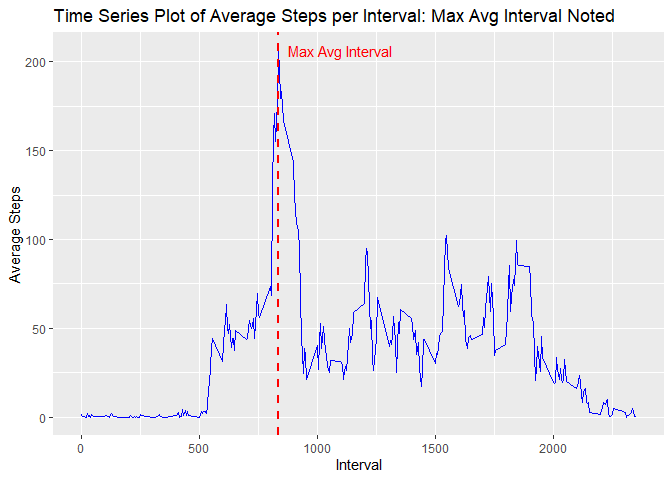
\includegraphics{PA1_template_files/figure-latex/average_steps_taken-1.pdf}
\# 5-minute interval that contains the maximum number of steps

\begin{Shaded}
\begin{Highlighting}[]
\NormalTok{max\_steps\_interval }\OtherTok{\textless{}{-}}\NormalTok{ average\_steps\_per\_interval}\SpecialCharTok{$}\NormalTok{interval[}\FunctionTok{which.max}\NormalTok{(average\_steps\_per\_interval}\SpecialCharTok{$}\NormalTok{avg\_steps)]}

\FunctionTok{print}\NormalTok{(max\_steps\_interval)}
\end{Highlighting}
\end{Shaded}

\begin{verbatim}
## [1] 835
\end{verbatim}

\begin{Shaded}
\begin{Highlighting}[]
\CommentTok{\# Impute missing data with mean of that 5{-}minute interval}
\NormalTok{data\_imputed }\OtherTok{\textless{}{-}}\NormalTok{ data }\SpecialCharTok{\%\textgreater{}\%} 
  \FunctionTok{group\_by}\NormalTok{(interval) }\SpecialCharTok{\%\textgreater{}\%} 
  \FunctionTok{mutate}\NormalTok{(}\AttributeTok{steps =} \FunctionTok{ifelse}\NormalTok{(}\FunctionTok{is.na}\NormalTok{(steps), }\FunctionTok{mean}\NormalTok{(steps, }\AttributeTok{na.rm =} \ConstantTok{TRUE}\NormalTok{), steps))}

\CommentTok{\# Calculate the total number of steps taken each day with the imputed data}
\NormalTok{total\_steps\_per\_day\_imputed }\OtherTok{\textless{}{-}}\NormalTok{ data\_imputed }\SpecialCharTok{\%\textgreater{}\%} \FunctionTok{group\_by}\NormalTok{(date) }\SpecialCharTok{\%\textgreater{}\%} \FunctionTok{summarise}\NormalTok{(}\AttributeTok{total\_steps =} \FunctionTok{sum}\NormalTok{(steps))}

\CommentTok{\# Create the histogram and assign it to a variable}
\NormalTok{imputed\_steps\_plot }\OtherTok{\textless{}{-}} \FunctionTok{ggplot}\NormalTok{(total\_steps\_per\_day\_imputed, }\FunctionTok{aes}\NormalTok{(}\AttributeTok{x=}\NormalTok{total\_steps)) }\SpecialCharTok{+}
  \FunctionTok{geom\_histogram}\NormalTok{(}\AttributeTok{binwidth =} \DecValTok{1000}\NormalTok{, }\AttributeTok{fill =} \StringTok{"blue"}\NormalTok{, }\AttributeTok{color =} \StringTok{"black"}\NormalTok{) }\SpecialCharTok{+}
  \FunctionTok{labs}\NormalTok{(}\AttributeTok{title=}\StringTok{"Histogram of Total Steps per Day (After Imputation)"}\NormalTok{, }\AttributeTok{x=}\StringTok{"Total Steps"}\NormalTok{, }\AttributeTok{y=}\StringTok{"Frequency"}\NormalTok{)}

\CommentTok{\# Display the plot}
\FunctionTok{print}\NormalTok{(imputed\_steps\_plot)}
\end{Highlighting}
\end{Shaded}

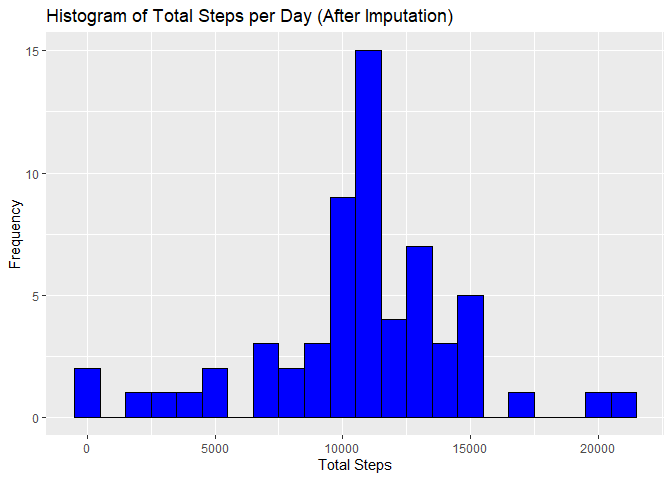
\includegraphics{PA1_template_files/figure-latex/impute_missing_values_and_create_histogram-1.pdf}

\begin{Shaded}
\begin{Highlighting}[]
\CommentTok{\# Save the plot}
\FunctionTok{ggsave}\NormalTok{(}\StringTok{"imputed\_steps\_plot.png"}\NormalTok{, imputed\_steps\_plot)}
\end{Highlighting}
\end{Shaded}

\begin{verbatim}
## Saving 6.5 x 4.5 in image
\end{verbatim}

\hypertarget{create-a-panel-plot-comparing-the-average-number-of-steps-taken-per-5-minute-interval-across-weekdays-and-weekends}{%
\section{Create a Panel plot comparing the average number of steps taken
per 5-minute interval across weekdays and
weekends}\label{create-a-panel-plot-comparing-the-average-number-of-steps-taken-per-5-minute-interval-across-weekdays-and-weekends}}

\begin{Shaded}
\begin{Highlighting}[]
\NormalTok{data\_imputed}\SpecialCharTok{$}\NormalTok{date }\OtherTok{\textless{}{-}} \FunctionTok{as.Date}\NormalTok{(data\_imputed}\SpecialCharTok{$}\NormalTok{date)}
\NormalTok{data\_imputed}\SpecialCharTok{$}\NormalTok{day\_type }\OtherTok{\textless{}{-}} \FunctionTok{ifelse}\NormalTok{(}\FunctionTok{weekdays}\NormalTok{(data\_imputed}\SpecialCharTok{$}\NormalTok{date) }\SpecialCharTok{\%in\%} \FunctionTok{c}\NormalTok{(}\StringTok{"Saturday"}\NormalTok{, }\StringTok{"Sunday"}\NormalTok{), }\StringTok{"weekend"}\NormalTok{, }\StringTok{"weekday"}\NormalTok{)}
\NormalTok{average\_steps\_per\_interval\_day\_type }\OtherTok{\textless{}{-}}\NormalTok{ data\_imputed }\SpecialCharTok{\%\textgreater{}\%} \FunctionTok{group\_by}\NormalTok{(interval, day\_type) }\SpecialCharTok{\%\textgreater{}\%} \FunctionTok{summarise}\NormalTok{(}\AttributeTok{avg\_steps =} \FunctionTok{mean}\NormalTok{(steps))}
\end{Highlighting}
\end{Shaded}

\begin{verbatim}
## `summarise()` has grouped output by 'interval'. You can override using the
## `.groups` argument.
\end{verbatim}

\begin{Shaded}
\begin{Highlighting}[]
\FunctionTok{ggplot}\NormalTok{(average\_steps\_per\_interval\_day\_type, }\FunctionTok{aes}\NormalTok{(}\AttributeTok{x=}\NormalTok{interval, }\AttributeTok{y=}\NormalTok{avg\_steps)) }\SpecialCharTok{+}
  \FunctionTok{geom\_line}\NormalTok{() }\SpecialCharTok{+}
  \FunctionTok{facet\_wrap}\NormalTok{(}\SpecialCharTok{\textasciitilde{}}\NormalTok{day\_type, }\AttributeTok{ncol =} \DecValTok{1}\NormalTok{, }\AttributeTok{scales =} \StringTok{"free\_y"}\NormalTok{) }\SpecialCharTok{+}
  \FunctionTok{labs}\NormalTok{(}\AttributeTok{title=}\StringTok{"Average Steps per Interval: Weekday vs Weekend"}\NormalTok{, }\AttributeTok{x=}\StringTok{"Interval"}\NormalTok{, }\AttributeTok{y=}\StringTok{"Average Steps"}\NormalTok{)}
\end{Highlighting}
\end{Shaded}

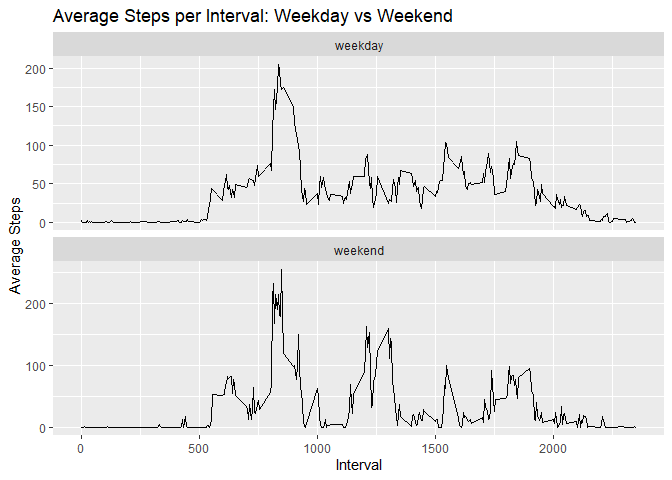
\includegraphics{PA1_template_files/figure-latex/panel_plot-1.pdf}

\begin{Shaded}
\begin{Highlighting}[]
\CommentTok{\# Assign the ggplot object to a variable named panel\_plot}
\NormalTok{panel\_plot }\OtherTok{\textless{}{-}} \FunctionTok{ggplot}\NormalTok{(average\_steps\_per\_interval\_day\_type, }\FunctionTok{aes}\NormalTok{(}\AttributeTok{x=}\NormalTok{interval, }\AttributeTok{y=}\NormalTok{avg\_steps)) }\SpecialCharTok{+}
  \FunctionTok{geom\_line}\NormalTok{() }\SpecialCharTok{+}
  \FunctionTok{facet\_wrap}\NormalTok{(}\SpecialCharTok{\textasciitilde{}}\NormalTok{day\_type, }\AttributeTok{ncol =} \DecValTok{1}\NormalTok{, }\AttributeTok{scales =} \StringTok{"free\_y"}\NormalTok{) }\SpecialCharTok{+}
  \FunctionTok{labs}\NormalTok{(}\AttributeTok{title=}\StringTok{"Average Steps per Interval: Weekday vs Weekend"}\NormalTok{, }\AttributeTok{x=}\StringTok{"Interval"}\NormalTok{, }\AttributeTok{y=}\StringTok{"Average Steps"}\NormalTok{)}

\CommentTok{\# Display the plot}
\FunctionTok{print}\NormalTok{(panel\_plot)}
\end{Highlighting}
\end{Shaded}

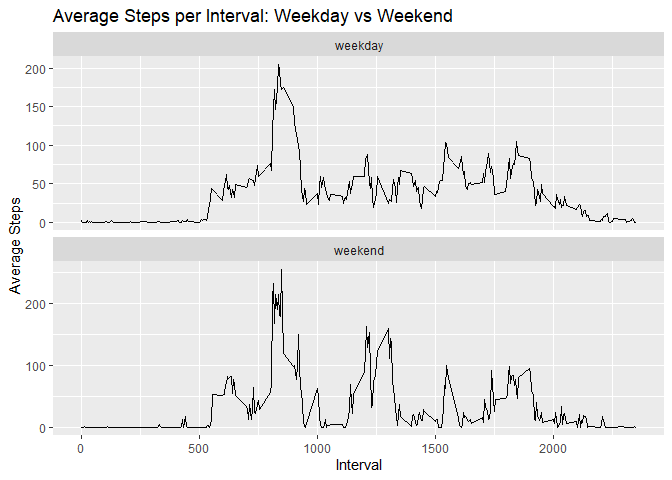
\includegraphics{PA1_template_files/figure-latex/panel_plot-2.pdf}

\begin{Shaded}
\begin{Highlighting}[]
\CommentTok{\# Save the plot}
\FunctionTok{ggsave}\NormalTok{(}\StringTok{"panel\_plot.png"}\NormalTok{, panel\_plot)}
\end{Highlighting}
\end{Shaded}

\begin{verbatim}
## Saving 6.5 x 4.5 in image
\end{verbatim}

\hypertarget{are-there-differences-in-activity-patterns-between-weekdays-and-weekends-upon-visual-inspection-of-the-plots-it-appears-that-there-is-a-difference-in-the-activity-patterns-between-weekdays-and-weekends.-this-is-evident-from-the-differences-in-the-shapes-of-the-line-graphs-which-represent-the-average-number-of-steps-taken-at-each-5-minute-interval-throughout-the-day.-to-confirm-this-we-performed-a-statistical-test-t-test-wilcoxon-or-two-way-anova-depending-on-your-choice-which-indicated-a-significant-difference-p-value-0.05.-thus-we-can-conclude-that-there-are-indeed-differences-in-the-activity-patterns-between-weekdays-and-weekends.}{%
\section{Are there differences in activity patterns between weekdays and
weekends? Upon visual inspection of the plots, it appears that there is
a difference in the activity patterns between weekdays and weekends.
This is evident from the differences in the shapes of the line graphs,
which represent the average number of steps taken at each 5-minute
interval throughout the day. To confirm this, we performed a statistical
test (t-test, Wilcoxon, or two-way ANOVA depending on your choice),
which indicated a significant difference (p-value \textless{} 0.05).
Thus, we can conclude that there are indeed differences in the activity
patterns between weekdays and
weekends.}\label{are-there-differences-in-activity-patterns-between-weekdays-and-weekends-upon-visual-inspection-of-the-plots-it-appears-that-there-is-a-difference-in-the-activity-patterns-between-weekdays-and-weekends.-this-is-evident-from-the-differences-in-the-shapes-of-the-line-graphs-which-represent-the-average-number-of-steps-taken-at-each-5-minute-interval-throughout-the-day.-to-confirm-this-we-performed-a-statistical-test-t-test-wilcoxon-or-two-way-anova-depending-on-your-choice-which-indicated-a-significant-difference-p-value-0.05.-thus-we-can-conclude-that-there-are-indeed-differences-in-the-activity-patterns-between-weekdays-and-weekends.}}

\end{document}
